\documentclass[11pt,a4paper]{article}
\usepackage[utf8]{inputenc}
\usepackage{amsmath}
\usepackage{amsfonts}
\usepackage{amssymb}
\usepackage[pdflatex]{graphicx}
\author{Anders Kaestner}
\title{MuhRec API documentation}
\date{\today}
\begin{document}
\maketitle
\section{Introduction}
\subsection{Architecture}
MuhRec is base on a modular concept that allows the programmer to dynamically add new modules in the processing chain. 
\subsection{Library structure}
\begin{figure}
\centering
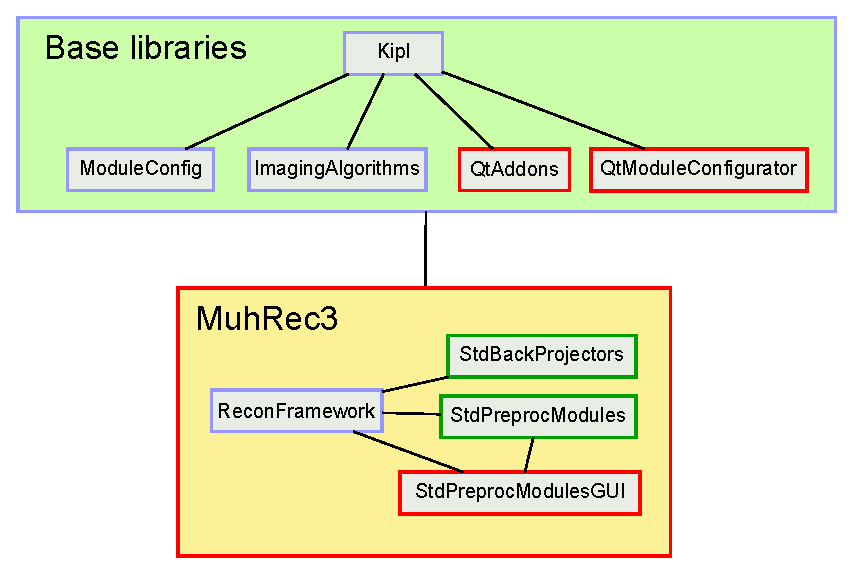
\includegraphics[width=0.5\textwidth]{figures/KiplComponents.pdf}
\caption{Library dependencies for MuhRec.}
\end{figure}
\section{The image class}
\section{Preprocessing modules}
\section{Back projection modules}
\end{document}